
\textbf{Completion of sinusoids.} We start with a simple example where LLMs extrapolate a function of the form $f(x) = a \cdot\sin{(bx)}$. As in \cref{sec:sequence_transformation}, tokenization matters; we found it effective to discretize outputs among integers 0--100, as these integers are represented by single tokens in the tokenizers of the LLMs we tested.

\begin{wrapfigure}{r}{0.48\textwidth}
    \vspace{-1.5em}
    \centering
    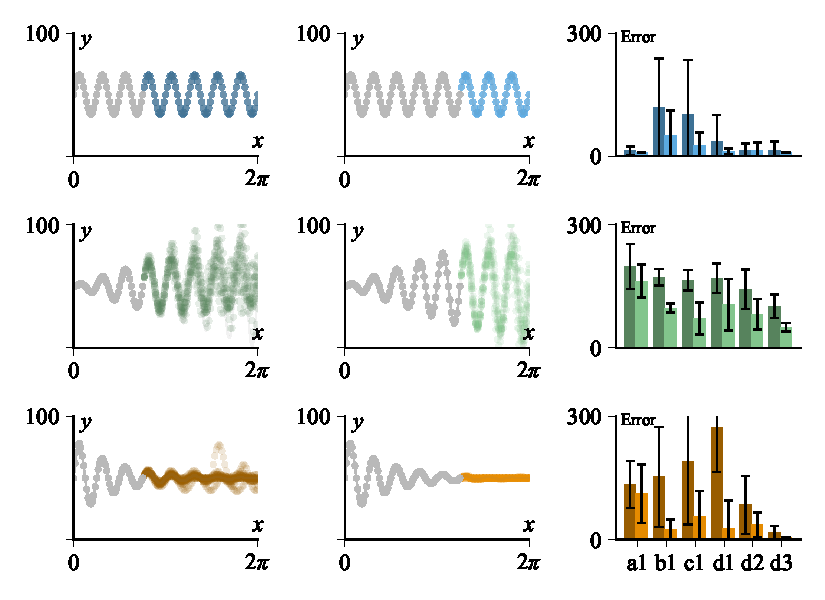
\includegraphics[width=1\textwidth]{figures/sinusoid-v1.pdf}
    \captionof{figure}{\small
    LLMs (d3 shown) can extrapolate various functions  $y=a\cdot\sin{(bx)}$ (top row), $y=ax\cdot\sin{(bx)}$ (middle row), and $y=\frac{a}{2^x}\sin{(bx)}$ (bottom row) given amounts of context. Overall, larger models make better predictions with lower error rates (right column). More context also helps prediction accuracy (light vs. dark).
    \vspace{-.5em}
    }
    \vspace{-1.3em}
    \label{fig:sinusoid}
\end{wrapfigure}

\cref{fig:sinusoid} shows completions of the sine wave by text-davinci-003 over 11 trials given 3 and 5 periods as context, as well as average distance (computed by Dynamic Time Warping) of the generated predictions to the ground truth function values across several LLMs. Multiple LLMs produce near-perfect continuations of the sine wave, especially with more context (\ie more periods of the sine wave). We additionally test the function family $ax \cdot\sin{(bx)}$---in which the amplitude of the oscillations increases with $x$-values. Here, the LLM must extrapolate to new values unseen in the context, which highlights the utility of using a metric space for the outputs (0--100) where the LLM has priors over the scale of the different tokens. These functions also contain a ``meta-pattern'': the $y$-values increase, decrease, and then increase in a single period---and the amplitude of the function also increases over time. This is a form of least-to-most prompting \cite{zhou2022least}, an ability we find useful later for sequence improvement in \cref{sec:sequence_improvement}.
We also test the function $\frac{a}{2^x} \cdot\sin{(bx)}$. Across these three functions, we observe that greater context and larger scale LLMs yield higher quality predictions. %



\textbf{Completion of periodic motions.} We emphasize that the Sequence Completion capability above is domain-agnostic---\ie we do not use any specialized prompts explaining what function should be completed, nor do we provide any linguistic grounding for the metric tokens. We can therefore operationalize this zero-shot capability of LLMs to simple open-loop motion extrapolation problems in robotics, \eg by encoding a series of positions sampled from a demonstration, and predicting future positions. We test two simple tasks on a mobile robot manipulator: \textit{Table Sweeping} and \textit{Whiteboard Drawing} (both shown in \cref{fig:teaser}).

In \textit{Table Sweeping}, the goal is to continue a human-provided kinesthetic demonstration of sweeping a portion of a table (see middle \cref{fig:teaser}). We encode the demonstration as a series of end-effector poses at approximately 3 Hz. Each demonstration lasts roughly 20-30 seconds. We represent the 7-dim end-effector pose as a concatenation of Cartesian position and the quaternion, where each value is binned to an integer between 0 and 100, and the dimensions are delimited by spaces. We collect 30 demonstrations that demonstrate the sweeping motion. Note that demonstrations in this task are noisier and higher dimensional than the stylized sinusoid functions above. For each demonstration, we construct a context to consist of the first two-thirds of the provided demonstration, and treat the last one-third as the ground truth for the LLM to predict. Larger models quantitatively perform better with generally lower variance (see Appendix).

In \textit{Whiteboard Drawing}, the goal is to continue a scripted demonstration of drawing loops on a whiteboard (see \cref{fig:teaser}). Loops are defined by parametric equations of the form $x = a_x \cos(bt) + d_x$ and $y = a_y \sin(bt) + c_y t + d_y$. We execute the motions using position control and record the end-effector positions at 5 Hz, then discretize states in between 0 and 300, as finer motion is needed for this task. We provide part of the loop pattern in-context, and assess the ability to extrapolate from 2 loops to do a third loop. LLMs, \eg text-davinci-003 perform well---we show more completions with different loop styles in the Appendix.